%Figure file
% dont use _ or whitespace in tags
% every tag added here be sure to add into figtag.tex

\iflspCommEx% <lspCommEx>
\begin{figure}
    \begin{plantuml}
      @startuml
      skinparam defaultTextAlignment center
      skinparam SequenceMessageAlign center
      actor User
      participant DevTool
      participant LangServer
      activate User
      activate DevTool
      activate LangServer
      User -> DevTool: open document
      DevTool -> LangServer: Notification: textDocument/didOpen; Params: document
      User -> DevTool: edit document
      DevTool -> LangServer: Notification: textDocument/didChange; Params: {documentURI, changes}
      LangServer -> DevTool: Notification: textDocument/publishDiagnostics; Params: Diagnostic[]
      User -> DevTool: execute goto definition
      DevTool -> LangServer: Request: textDocument/definition; Params: {documentURI, position}
      LangServer -> DevTool: Response: textDocument/definition; Result: Location
      User -> DevTool: close document
      DevTool -> LangServer: Notification: textDocument/didClose; Params: documentURI
      deactivate LangServer
      deactivate DevTool
      deactivate User
      @enduml
    \end{plantuml}
    \caption{Example of communication between the LSP client and server \cite{lsp}}
    \label{lspCommEx}
\end{figure}
\fi% </lspCommEx>

\ifvsceArch% <vsceArch>
\begin{figure}
    \begin{plantuml}
      @startuml
      skinparam defaultTextAlignment center
      skinparam SequenceMessageAlign center
      skinparam linetype ortho
      left to right direction
        rectangle "VS Code" {
        rectangle "Extension Host" {
        rectangle hlc [
        HTML Language Client
        ]
        rectangle plc [
        PHP Language Client
        ]
        }
        }
        
        rectangle hls [
        HTML Language Server
        ]
        rectangle pls [
        PHP Language Server
        ]
        
        hlc --> hls
        hls --> hlc: LSP over JSON-RPC
        plc --> pls
        pls --> plc: LSP over JSON-RPC
      @enduml
    \end{plantuml}
    \caption{Integration of extension into VSCode\cite{vsclspextman}}
    \label{vsceArch}
\end{figure}
\fi% </vsceArch>

\ifdaGdb% <daGdb>
\begin{figure}
    \begin{plantuml}
    @startuml
      skinparam defaultTextAlignment center
      skinparam SequenceMessageAlign center
      actor User
      participant DevTool
      participant DebugAdapter
      participant Debugger
      User -> DevTool : start debugging
      activate DevTool
      DevTool -> DebugAdapter: start debug adapter
      activate DebugAdapter
      DevTool -> DebugAdapter: initialize request
      DebugAdapter -> Debugger: start gdb
      activate Debugger
      DebugAdapter -> DevTool: response: capabilities
      DebugAdapter --> DevTool: initalized event
      User -> DevTool : set breakpoint
      DevTool -> DebugAdapter: setBreakpoints request
      DebugAdapter -> Debugger: break "hello.c:main:4"
      DebugAdapter -> DevTool: response: breakpoints
      User -> DevTool : run
      DevTool -> DebugAdapter: launch request
      DebugAdapter -> Debugger: file "a.out"
      DebugAdapter -> Debugger: run
      DebugAdapter -> DevTool: response: status
      deactivate DevTool
      deactivate DebugAdapter
      deactivate Debugger
    @enduml
    \end{plantuml}
    \caption{Example of communication between IDE's generic debugger and GDB via Debug adapter \cite{dap}}
    \label{daGdb}
\end{figure}
\fi% </daGdb>

\ifmnProb% </mnProb>
\begin{figure}
    \begin{plantuml}
      @startuml
      skinparam defaultTextAlignment center
      skinparam linetype polyline
      left to right direction
      rectangle Languages {
        usecase "JS" as js
        usecase "Python" as py
        usecase "Java" as jav
      }
      rectangle IDEs {
        usecase "VSCode" as vsc
        usecase "Eclipse" as ec
        usecase "Vim" as vim
      }
      js --> vsc
      js --> ec
      js --> vim
      py --> vsc
      py --> ec
      py --> vim
      jav --> vsc
      jav --> ec
      jav --> vim
      @enduml
    \end{plantuml}
    \caption{The {\it m+n} problem\cite{vsclspextman}}
    \label{mnProb}
\end{figure}
\fi% </mnProb>

\ifsolMnProb% </solMnProb>
\begin{figure}
    \begin{plantuml}
      @startuml
      skinparam defaultTextAlignment center
      left to right direction
      rectangle LSP_Server {
        usecase "JS" as js
        usecase "Python" as py
        usecase "Java" as jav
      }
      rectangle LSP
      rectangle LSP_Client {
        usecase "VSCode" as vsc
        usecase "Eclipse" as ec
        usecase "Vim" as vim
      }
      js --> LSP
      py --> LSP
      jav --> LSP
      LSP --> vsc
      LSP --> ec
      LSP --> vim
      @enduml
    \end{plantuml}
    \caption{Solution to {\it m+n} problem\cite{vsclspextman}}
    \label{solMnProb}
\end{figure}
\fi% </solMnProb>

\ifsolDbg% </solDbg>
\begin{figure}
    \begin{plantuml}
      @startuml
      skinparam defaultTextAlignment center
      left to right direction
      rectangle "IDE (with Generic Debugger)" {
        usecase "VSCode" as vsc
        usecase "Eclipse" as ec
        usecase "Vim" as vim
      }
      rectangle DA
      rectangle JS_DA
      rectangle Python_DA
      rectangle Java_DA
      rectangle JS_Debugger
      rectangle Python_Debugger
      rectangle Java_Debugger
      vsc --> DA
      ec --> DA
      vim --> DA
      DA --> JS_DA
      DA --> Python_DA
      DA --> Java_DA
      JS_DA --> JS_Debugger 
      Python_DA --> Python_Debugger
      Java_DA --> Java_Debugger
      @enduml
    \end{plantuml}
    \caption{Solution for debugging support\cite{dap}}
    \label{solDbg}
\end{figure}
\fi% </solDbg>

\ifiro% </iro>
\begin{figure}
    \begin{plantuml}
      @startuml
      skinparam defaultTextAlignment center
      left to right direction
      rectangle IRO
      rectangle "Format" {
        usecase "Texmate" as tm
        usecase "Atom" as at
        usecase "Ace" as ace
        usecase "Sublime3" as sub3
      }
      rectangle "Users" {
        usecase "VSCode" as vsc
        usecase "Eclipse" as ec
        usecase "Github" as gh
        usecase "Atom editor" as atsh
        usecase "Ace editor" as acesh
        usecase "Sublime editor" as sub3sh
      }
      IRO --> tm
      IRO --> at
      IRO --> ace
      IRO --> sub3
      tm --> vsc
      tm --> ec
      tm --> gh
      at --> gh
      at --> atsh
      ace --> acesh
      sub3 --> sub3sh
      @enduml
    \end{plantuml}
    \caption{{\it IRO}\cite{iro} and supported grammar formats}
    \label{iro}
\end{figure}
\fi% </iro>

\ifauto% </auto>
\begin{figure}
    \begin{plantuml}
      @startuml
      skinparam defaultTextAlignment center
      package "Template project" as TPrj {
        [LSP Client with entry points]
        [LSP Server with entry points]
      }
      file "Entry point list YAML file" as EPY
      file "Language Configuration YAML file" as LCY
      rectangle "Automation script" {
      database "Automation script module" as AutoMod
      package "LSP project" as LSPrj {
        [LSP Client]
        [LSP Server]
      }
      database "npm installer" as npi
      package "Precompiled LSP project" as LSPPrj {
        [LSP Client]
        [LSP Server]
        [npm modules]
      }
      database "VSCE" as vsce
      }
      folder "LSP Extension" as LSPex  
      TPrj --> AutoMod
      EPY --> AutoMod
      LCY --> AutoMod
      AutoMod --> LSPrj
      LSPrj --> npi
      npi --> LSPPrj
      LSPPrj --> vsce
      vsce --> LSPex
      @enduml
    \end{plantuml}
    \caption{Automation of generation of LSP extension}
    \label{auto}
  \end{figure}
\fi% </auto>

\ifmyc% </myc>
\begin{figure}
    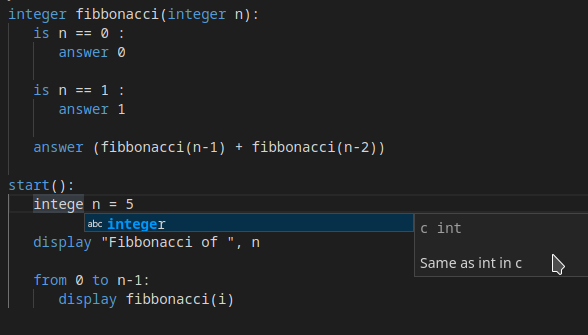
\includegraphics[width=\linewidth]{../fig/myc.png}
    \caption{Keyword syntax Highlighting, auto completion and inline documentation}
    \label{myc}
\end{figure}
\fi% </myc>

\ifmycext% </mycext>
\begin{figure}
    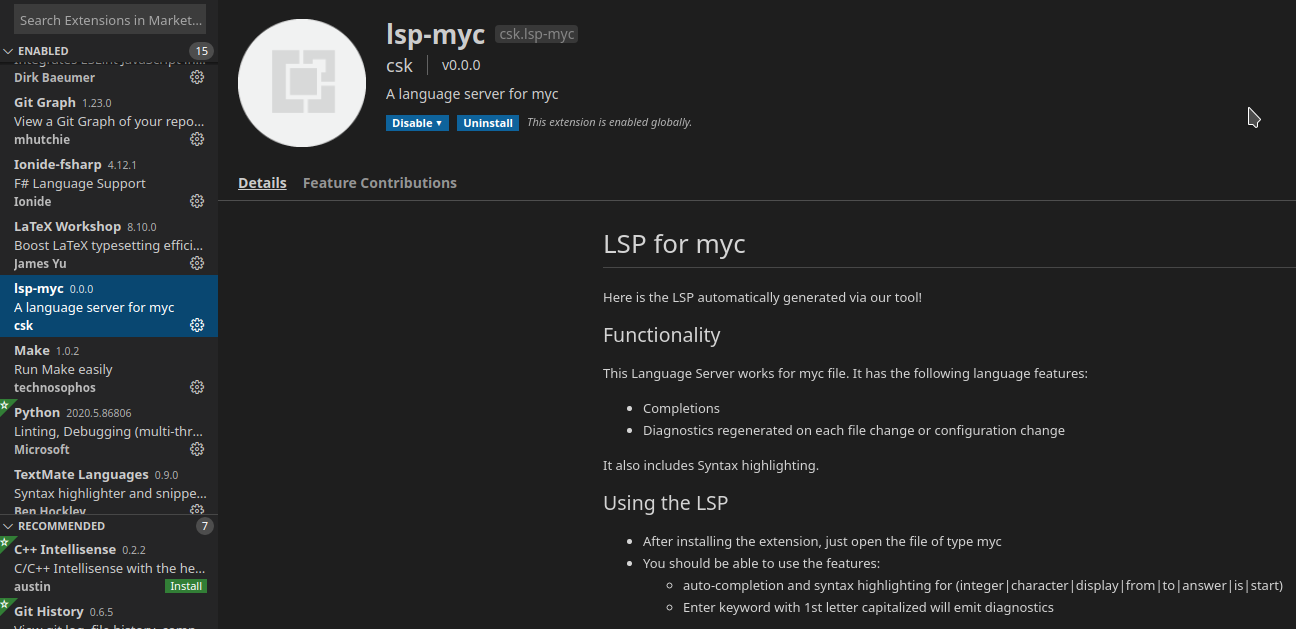
\includegraphics[width=\linewidth]{../fig/mycext.png}
    \caption{Extension for LSP of {\it myc} installed in VSCode}
    \label{mycext}
\end{figure}
\fi% </mycext>